\documentclass{article}

\usepackage[utf8]{inputenc}
\usepackage[spanish]{babel}
\usepackage{graphicx}

\title{Reporte Centro de Masa, Densidad de Fuentes I}


\author{W. P. Karel Zapfe}

\begin{document}

\maketitle


\section{La Señal Cruda}

El aparato, el BioCAM 4096S, es un arreglo de 4096 electrodos en un 
cuadrángulo con 64 renglones y 64 columnas en un cuadrado de
$(2.67 mm)^2$. Los electrodos permiten medir variaciones del orden
de unos micro-volts hasta aproximadamente 16 mili-volts 
en el potencial eléctrico de tejido colocado sobre el arreglo. Cuando
todos los electrodos están registrando actividad, tenemos una frecuencia de muestreo
de 7022 tomas por segundo. Cada electrodo tiene $21 \mu m$ de lado, lo
que hace que sus dimensiones sean del mismo orden de magnitud que el 
soma de una neurona piramidal típica. El aparato tiene, de acuerdo
con sus fabricantes, una señal ruidosa de $26 \mu V$rms. Dicha señal
está presente en todos los electrodos excepto en un par que se
muestran saturados todo el tiempo en varios registros.

Cuando una célula piramidal dispara se puede medir un cambio de potencial
en el medio extracelular. Si tomamos medidas \emph{muy} cercanas al soma
(menos de $25 \mu m$)
y no hay mas influencias, este cambio puede ser de aproximadamente
$-250\mu V$ \cite{Obien2015}. Poco después ocurre una repolarización
y se observa una señal contraria de aproximadamente $+100\mu V$.
Dado que el potencial decrece como el inverso de la distancia
y es aditivo, nuestras espigas discernibles en la señal tienen tamaños mucho
menores, pero distintamente arriba del nivel de ruido.

La actividad neuronal producirá una distribución diferente en las medidas
de los electrodos cercanos, mientras que aquellos que se encuentren
suficientemente alejados de las fuentes y sumideros de corriente
percibirán mayoritariamente ruido y tendrán otra estadística.
Esto nos permite separar los electrodos sobre los cuales
se encuentren cuerpos densamente llenos de células piramidales
de aquellas regiones vacías, y podremos identificar el CA.



\section{Limpiando la señal}

Para obtener una señal \emph{limpia} tenemos que tomar en cuenta
cual es nuestro propósito. Para realizar el estudio que está llevando a cabo
Franco basta con poder identificar las espigas del ruido.
Pero para poder obtener una densidad de fuentes de corriente esto no basta.
El procedimiento formal para obtener esta densidad, que denotaré
 por CSD, es calcular el \emph{Laplaciano} del potencial de
campo. Esto es un operador diferencial (la suma de las dobles derivadas 
cartesianas), y por ende requiere una \emph{función suave} para actuar. 
El Laplaciano es especialmente sensible al ruido, tanto así, que su
función en procesamiento de señales es detectar \emph{bordes duros}.
Esto es especialmente de interés para nosotros: su implementación
más común  se usa
justamente en la detección de bordes en imágenes  digitales.
El ruido es básicamente un montón de bordes duros en cada instante temporal.
Estamos obligados, por ende, a filtrar todo el ruido que sea posible.


\subsection{Identificando CA}

Una gran cantidad de electrodos se encuentran lejos de las células
piramidales y sólo registran ruido. Este ruido se puede caracterizar
por sus propiedades estadísticas. Un método común de separar secciones
en una imagen bidimensional que resulta fácil de implementar y que
da resultados sorprendentemente buenos es el llamado método de Otsu
\cite{Otsu79}.

A grandes rasgos, lo que hace la llamada ``umbralización de Otsu'' es
separar la señal bidimensional en dos conjuntos tales que su 
estadística sea \emph{lo más distante posible}, sin hacer ninguna
suposición al respecto de las características de cada señal.

Decidí confrontar una implementación de este método con
el método que usa Franco.
Rescaté algunas ideas de Franco para obtener una máscara que
revelara la parte del arreglo que nos interesa.
Los detalles de la implementación específica 
se encuentran en un \emph{notebook}. El resultado se muestra en la figura
\ref{OtsuMask}.  Toda señal fuera de esa máscara la trataremos como cero.

\begin{figure}[h]
  \centering
  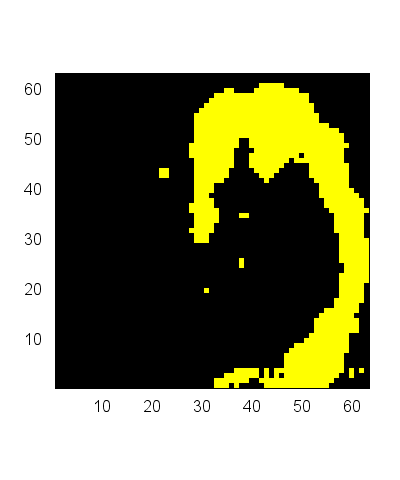
\includegraphics[width=0.45\textwidth]{MascaraOtsu01.png}
  \caption{Mascara obtenida mediante la suma sucesiva de varias
    umbralizaciones de Otsu. La figura amarilla cubre los electrodos
    que se encuentran cerca del cuerpo celular CA.} \label{OtsuMask}
\end{figure}  


\subsection{Quitando ruido}

La señal ruidosa se superpone a la señal de actividad neuronal en
los electrodos seleccionados. Una posibilidad para separarlas
sería utilizar las características de frecuencia de alguna de ambas 
y hacer pasar la señal de cada electrodo por un filtro pasa-bajos
o pasa-altos según sea el caso (Mario Treviño dixit).
Esto tiene un problema intrínseco: la señal ruidosa está acoplada
con la frecuencia de alternancia de la corriente, que en México es
de entre 55 a 65 Hz. Una espiga putativa en nuestra señal
(ver figura \ref{espiga}) tiene una estructura con duración
temporal de aproximadamente $5 ms$. Esto es aproximadamente 
un tercio del tamaño de la estructura asociada a los 60Hz,
asi que es demasiado cercana como para usarse confiadamente.
Preferí usar un simple criterio de umbral: todo aquello
que estuviera por debajo de $60\mu V$ en valor absoluto 
sería considerado ruido y transformado a ceros. La
comparación entre una señal original y la señal umbralizada
se muestra en la figura \ref{umbralc}.


\begin{figure}[h]
  \centering
  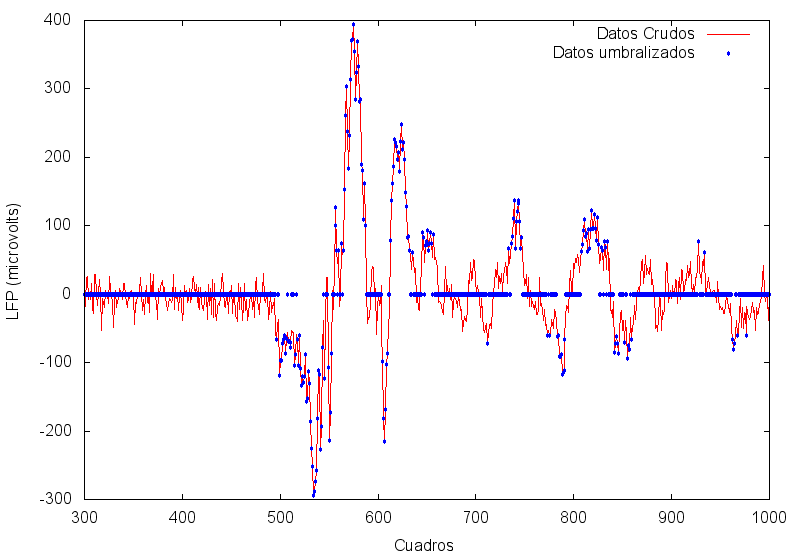
\includegraphics[width=0.75\textwidth]{ComparaUmbral.png}
  \caption{Mascara obtenida mediante la suma sucesiva de varias
    umbralizaciones de Otsu. La figura amarilla cubre los electrodos
    que se encuentran cerca del cuerpo celular CA.} \label{umbralc}
\end{figure}  


\subsection{Suavizando la señal}


La implementación directo del operador
Laplaciano discreto en una retícula bidimensional produce
efectos de borde muy notorios que ofuscarían la visualización
de las áreas con verdadera actividad. Es por ello que se
desarrollo un método de suavización de bordes en la  implementación
del operador llamado ``filtro Gauss-Laplace''. Consiste en pasar
un filtro Gaussiano por la imágen o señal primero, y luego el 
operador Laplaciano discreto. Esta fue la ``segunda derivada'' que
decidí implementar para buscar la densidad de fuentes de corrientes.
Esto producirá un efecto de señal de potencial similar a 
la de un campo apantallado, que es, hasta donde yo se,
 adecuada para modelar iones disueltos en un  medio
 complicado. Un ejemplo del efecto de cruz en esta resolución
 se puede ver en la figura \ref{LaplacianEfect}

\begin{figure}[h]
  \centering
  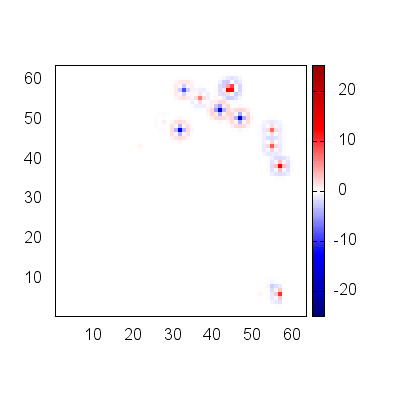
\includegraphics[width=0.45\textwidth]{EjemploLaplacian01.png}
  \caption{Efecto de ``cruz'' por la implementación del Laplaciano discreto
    en una malla de 64 por 64 píxeles. La escala es muy cercana al
  $\epsilon$ de la derivada. }\label{LaplacianEfect}
\end{figure}  

 
La señal ya así obtenida tiene todavía el inconveniente
de ser muy ``dura'' en el dominio espacial. Aunque $64\times 64$
puntos de muestreo en tan poco espacio tenga una resolución
alta en comparación con las estructuras fisiológicas, es baja
para obtener derivadas numéricas descentes.
Las gráficas obtenidas en Matlab por Treviño et all y Luzdas et all
se muestran mucho más suaves al calcular la CSD. Esto es escencialmente
debido a que Matlab interpola valores entre puntos de la malla
para crear un gradiante suave de colores. Si vamos a usar una
interpolación, es conveniente que usemos una que no aporte información
espuria a los datos y que podamos controlar los parámetros directamente.
Para ello usaremos una rutina de interpolación cuadrática
(que garantiza la existencia de segundas derivadas) y condiciones
en la frontera que extiendan el último renglón o fila.



\section{Centros de Masa}



\bibliographystyle{plain}

\bibliography{BiblioReportes01}














\end{document}
